\documentclass[conference]{IEEEtran}
\usepackage{fancybox}
\usepackage{cite}
\usepackage{float}
\usepackage{Sweavel}
\usepackage{xspace}
\usepackage{placeins}
\usepackage{tikz}
\usetikzlibrary{calc,trees,positioning,arrows,fit,shapes,calc,cd}
\usepackage{tkz-kiviat} 
\usepackage{pgfplots} 
\usetikzlibrary{arrows}
\usepackage{amssymb}
\usepackage{caption}
 
\usepackage{algpseudocode}
\usepackage{algorithm}
\usepackage{algorithmicx}
\newcommand{\theHalgorithm}{\arabic{algorithm}}

\def\mytitle{Avoiding The Impact of Equivalent Mutants With Second Degree Kills}
 
\usepackage[bookmarks=true, urlcolor=blue, linkcolor=blue, citecolor=blue, colorlinks=true, pdftitle={\mytitle}, pdfauthor={Rahul Gopinath}]{hyperref}

\usepackage{comment}

\usepackage{listings}
\usepackage{float}
\floatstyle{plain}
\newfloat{program}{t}{lop}
\floatname{program}{Figure}
\usepackage{color}

\definecolor{dkgreen}{rgb}{0,0.6,0}
\definecolor{gray}{rgb}{0.5,0.5,0.5}
\definecolor{mauve}{rgb}{0.58,0,0.82}

\lstset{frame=tb,
  language=Java,
  aboveskip=3mm,
  belowskip=3mm,
  showstringspaces=false,
  columns=flexible,
  basicstyle={\footnotesize\ttfamily},
  numbers=left,
  numberstyle=\tiny\color{gray},
  keywordstyle=\color{blue},
  commentstyle=\color{dkgreen},
  stringstyle=\color{mauve},
  breaklines=true,
  breakatwhitespace=true
  tabsize=3
}
\usepackage{color}
\definecolor{lightgray}{gray}{0.75}

\newcommand\greybox[1]{  \vskip\baselineskip  \par\noindent\colorbox{lightgray}{  \begin{minipage}{0.99\columnwidth}#1\end{minipage}  }  \vskip\baselineskip}

\newcommand{\minM}{M^{\mu}}
\newcommand{\surfaceM}{M^{\rho}}
\newcommand{\surfaceC}{\rho}
\newcommand{\uniqM}{M^{\delta}}
 


\ifCLASSINFOpdf
            \else
                  \fi





\usepackage[cmex10]{amsmath}










































\hyphenation{op-tical net-works semi-conduc-tor}
\newcounter{observation}
\newcommand{\observation}[1]{\refstepcounter{observation}

	\begin{center}
	\Ovalbox{
	\begin{minipage}{0.93\columnwidth}
		\textbf{Observation \arabic{observation}:} #1
		\end{minipage}
		}
		\end{center}
		\vspace{-5pt}
}


\begin{document}
\title{\mytitle}


\author{
\IEEEauthorblockN{
Rahul Gopinath\IEEEauthorrefmark{1},
Iftekhar Ahmed\IEEEauthorrefmark{2},
Amin Alipour\IEEEauthorrefmark{3},
Carlos Jensen\IEEEauthorrefmark{4}, and
Alex Groce\IEEEauthorrefmark{5}}
\IEEEauthorblockA{Department of EECS, Oregon State University\\
Email: \IEEEauthorrefmark{1}gopinath@eecs.orst.edu,
\IEEEauthorrefmark{2}ahmed@eecs.orst.edu,
\IEEEauthorrefmark{3}alipour@eecs.orst.edu,
\IEEEauthorrefmark{4}cjensen@eecs.orst.edu,
\IEEEauthorrefmark{5}agroce@gmail.com
}}
 









\maketitle


\begin{abstract}
Mutation analysis assesses the quality of test suites by
evaluating them against an exhaustive set of generated faults.
Mutation analysis is vulnerable to mutant clones which differ from one
another syntactically but not semantically. Equivalent and
redundant mutants induce skew in mutation scores making the measure
less trustworthy.

We show that a simple modification of mutation analysis,
trading speed for accuracy, can avoid many of the problems due to
mutant clones that plague mutation analysis. We propose using
a new measure $\mu_2$ --- the ratio between mutants killed at least
twice ($M_2$) to those killed at least once ($M_1$). We show that
our new measure $\mu_2$ reaches unity at the same time as the
traditional mutation score $\mu_1$, and is monotonic with the
effectiveness of the test suite. We also show that the
odds ratio for $n^{th}$-degree mutation scores for any project increases
linearly with $n$, and they all approach unity in the limit.

Our new measure has two key advantages. It avoids the problem of
equivalent mutants, and being defined statistically, it also avoids
the problem of redundant mutants. It may also be used to predict
the traditional mutation score of a project accurately.
 \end{abstract}





\IEEEpeerreviewmaketitle


\newcommand*\per{\scalebox{.5}{\%}}
\begin{comment}


\end{comment}



\setlength\tabcolsep{2pt}





\section{Introduction}

Software testing is the primary means of ensuring quality of software
systems, and mutation analysis~\cite{lipton1971fault,budd1979mutation} is the
premier means of assessing and comparing the quality of test suites. 

Mutation analysis involves \emph{exhaustive} generation of first order syntactic
faults which are then tested against a given test suite. The ratio of
faults (mutations) detected by a test suite to the total faults generated is thought
to correlate with the ability of a test suite to find real faults.
Daran et al.~\cite{daran1996software}, suggest that faults generated by
first order mutations are comparable to real world faults in terms of error
traces produced.  Andrews et al.~\cite{andrews2005mutation,andrews2006using},
found that faults generated by mutation analysis have similar in detectability
to real world faults (in comparison to hand seeded
faults). Do et al.~\cite{do2006on} showed that using mutation faults for test
prioritization result in higher fault detection rates than using hand seeded faults.
Li et al.~\cite{li2009experimental} showed that while comparing four adequacy
criteria --- mutation, edge pair, all uses, and prime path ---
mutation adequate testing was able to detect most the hand seeded faults (85\%)
compared to other criteria (65\%).
Finally, Just et al.~\cite{just2014mutants} empirically showed that
effectiveness of a test suite in detection of mutants mirrors its ability to
detect real faults.

One of the key concerns in mutation analysis is the ability to distinguish
equivalent mutants.
Equivalent mutants are those mutants which differ from the
original syntactically, but not semantically.
The true mutation score is given by
\[
\mu_{true} = \frac{|M_{killed}|}{|M_{killable}|}\; \bigg| M_{killable} = M_{generated} - M_{equivalent}
\]

As the equation shows, the accuracy of a mutation score depends on identifying
the equivalent mutants correctly.
Undetected equivalent mutants deflate the mutation score artificially, making
assessment of test suite quality difficult. It also reduces confidence in
the mutation score because the distribution of equivalent mutants in software
is unknown, and hence it is difficult to estimate the adequacy of a test suite
--- whether all mutants that are killable have been killed, and if the
remaining mutants could be killed by enhancing the test suite. 
However, a complete solution to equivalent mutants is prevented by Rice's
theorem~\cite{rice1953classes} which claims that a generalized solution to
comparing two programs (and hence distinguishing equivalent mutants from
actual mutants) is undecidable.

A similar problem is the problem of redundant mutants. A mutant is
redundant when the failures it causes are the same as the failures
that another (syntactically different) mutant causes. That is, it is
not necessary to execute both to determine the results (if a test
kills one, it kills the other). The  presence of redundant (and
detected) mutants tends to inflate the mutation score.  As with equivalent mutants, a general
solution to redundant mutants is undecidable.  

We mitigate the problems of equivalent and redundant mutants by
proposing an alternative to the traditional mutation score that
requires additional runtime but gains accuracy by reducing the impact
of equivalent and redundant mutants.

\greybox{ Say $M_{n}$
  is the set of mutants that were killed by \textbf{at least} $n$ test
  cases.  We define $n^{th}$ degree mutation score $\mu_n$ as the
  ratio $\frac{M_{n}}{M_{n-1}}$.  The traditional mutation score
  $\frac{M_{1}}{M_{0}}$ is the $1^{st}$ degree mutation score $\mu_1$.  }
Our approach sidesteps the problem of mutant clones by tackling the
issue statistically.  We show that the \emph{odds ratio} $M_n$ to
$M_{n-1}$ increases linearly with $n$, and that the ratio $\mu_n$ can
be estimated from $\mu_{n+1}$. We show that the difference between
$\mu_2$ and $\mu_3$ decreases as the adequacy of the test suite
increases, with both becoming arbitrarily close to 1.

This means that, for an adequate test suite, we expect the ratio $\mu_2$
to be $1$ or very close to $1$, and $\mu_2$ can serve as an
ideal substitute for $\mu_{true} = \mu_1 = \frac{M_1}{M_0}$ where $M_0$ is the total
killable mutants (excluding equivalents). Note that we do not need to worry
about problems due to redundant mutants because our definition is statistical
in nature. Secondly, we do not have to bother about equivalent mutants since by
definition we look only at mutants that are killed.

Our empirical evidence is presented in two parts. In the first part, we
evaluate 25 projects with large test suites using three
different mutation analysis tools for Java --- Pit, Judy, and Major. In the
second part, we evaluate a separate large project --- Apache
commons-math --- in detail, and show that our conclusions remain even
in the case of single projects, and are not an artifact of statistical evaluation
over numerous projects.

We caution that our empirical evidence is statistical. That is, it is
possible for pathological mutant distributions and test suites to exist.
However, our samples are drawn from numerous projects, giving 
strong confidence that such pathological projects and test suites
are rare in practice. Further, the possibility of pathological distributions
decrease as the size of the program being examined increase, and it is in these
large programs that mutation analysis is most useful.




\section{Related Work}
\label{sec:related}
Traditional mutation analysis involves exhaustive analysis of first order
faults, whose rate of detection by a test suite indicates the effectiveness
of the test suite~\cite{demillo1978hints}.  Mutation analysis relies on two fundamental
assumptions for its validity --- \emph{the competent programmer hypothesis},
and \emph{the coupling effect}. The competent programmer hypothesis suggests
that programmers make simple mistakes. That is,
we expect faulty programs to be in the close syntactic neighborhood of the
correct program. The coupling hypothesis suggests that test cases capable of
detecting a simple fault in isolation will be able to detect it even when the
fault appears in conjunction with other faults. That is, the semantic footprint
of a fault rarely reduces when it joins with other faults. 
Evidence of the coupling effect comes from theoretical analysis by
Wah~\cite{wah2000atheoretical,wah2003ananalysis}  and empirical studies by
Offutt~\cite{offutt1989thecoupling,offutt1992investigations}, and
Langdon et al.~\cite{langdon2010efficient}.
While the competent programmer hypothesis is harder to verify, the mean syntactic
difference between faults was quantified in our previous work~\cite{gopinath2014mutations}.

The technique of mutation analysis first proposed by
Lipton~\cite{lipton1971fault} et al., was formalized and refined by
DeMillo et al.~\cite{demillo1978hints}, and was
first implemented by Budd~\cite{budd1980theoretical} for his PhD thesis.
Mutation analysis was shown to subsume multiple coverage
measures including
\textit{statement}, \textit{branch}, and \textit{all-defs} dataflow
coverage~\cite{budd1980mutation,mathur1994empirical,offutt1996subsumption}.
The validity of mutation analysis was verified first by
Daran et al.~\cite{daran1996software} who found that the error traces produced
by mutants were similar to those produced by real faults. Additional evidence
from Andrews et al.~\cite{andrews2005mutation,andrews2006using} suggests
that the ease of detection for mutants is similar to real faults (and
dissimilar to hand seeded faults).
According to Do et al.~\cite{do2006on}, using mutation faults for test
prioritization results in higher fault detection rates than hand seeded faults.
Li et al.~\cite{li2009experimental} compared four adequacy criteria ---
mutation, edge pair, all uses, and prime path, and found that
mutation adequate testing was able to detect most hand seeded faults (85\%)
compared to others (65\%).
Finally, Just et al.~\cite{just2014mutants} using 357 real bugs showed that 1) adding more
fault-detecting tests to a test suite led to its mutant score being increased
more often (73\%) than either branch (50\%) or statement coverage (30\%)
and 2) mutation score is more positively correlated with fault detection.

Since the number of mutants produced during mutation analysis is very large,
and each mutant requires a full test suite run for evaluation, the runtime
requirements for mutation analysis are high. Research into
reducing the cost of mutation analysis is broadly categorized as
\textit{do smarter}, \textit{do faster}, and \textit{do fewer} by
Offutt et al.~\cite{offutt2001mutation}.
The \textit{do smarter} approaches include space-time trade-offs, weak
mutation analysis, and parallelization of mutation analysis. The \textit{do
faster} approaches include mutant schema generation, code patching, and
other methods to make mutation analysis faster as a whole. Finally, the
\textit{do fewer} approaches try to reduce the number of mutants examined,
and include selective mutation and mutant sampling.

Researchers have tried to approximate the full mutation score without
running a full mutation analysis. Using only a subset of mutants -- just 10\% --
(\textit{do fewer}) was suggested first by Budd~\cite{budd1980mutation}
and Acree~\cite{acree1980mutation} who showed that using this sufficient to
achieve 99\% accuracy of prediction for the final mutation score.
Further confirmation was provided by Mathur~\cite{mathur1991performance},
Wong et al.~\cite{wong1993mutation,wong1995reducing}, and Offutt et
al.~\cite{offutt1993experimental} using the Mothra~\cite{demillo1988an} mutation
operators for FORTRAN.  Lu Zhang et al.~\cite{zhang2010isoperator} compared
operator-based mutant selection techniques to random mutant sampling,
and found that random sampling performs as well as the operator selection
methods.  Lingming Zhang et al.~\cite{zhang2013operator} compared various
forms of sampling such as stratified random sampling based on operator strata,
stratified random sampling based on program element strata, and a combination
of the two. They found that stratified random sampling when strata were
used in conjunction performed best in predicting the final mutation score,
and as few as 5\% mutants was sufficient sample for a 99\% correlation with the actual
mutation score. Recently, it was found~\cite{gopinath2015howhard} that $9,604$
mutants were sufficient for obtaining $1\%$ accuracy for $99\%$ of the projects,
irrespective of the independence of mutants, or their total population.

A major theoretical (and practical) difficulty in mutation analysis is identifying
equivalent mutants --- mutants that are syntactically different, but
semantically indistinguishable from the original program, leading to incorrect
mutation scores.  In general, identifying equivalent mutants is
undecidable as a consequence of Rice's theorem~\cite{rice1953classes}. Further,
as Acree~\cite{acree1980mutation} shows, even human analysis may be only 80\%
correct, with 12\% chance of mislabeling equivalent mutants as killable, and 8\%
chance of labeling killable mutants as equivalent.
Work on ameliorating the impact of equivalent mutants is
generally divided into categories of prevention and detection~\cite{papadakis2015trivial}, with
prevention focusing on reducing the incidence of equivalent mutants
and detection focusing on identifying equivalent mutants by
examining their static and dynamic properties.
The effort at prevention include efforts to identify the operators most likely
to produce equivalent mutants. Yao et al.~\cite{yao2014astudy} evaluated the
equivalence of mutants manually. They found that most equivalent mutants caused
little state change. Further, they also found that the number of equivalent
mutants and the number of mutants that remain but are killable are not always
correlated, with equivalent mutants strongly correlated with total number of
mutants. In their study, equivalent mutants accounted for 23\% of all mutants
on average, while the undetected but killable mutants were only 7\% on average
after evaluation using a \emph{branch coverage adequate} test suite. They
found that the number of equivalent mutants in projects varies widely from 17\%
to 48\% of all mutants. They also found that some operators tend to produce
numerous equivalent mutants compared to undetected but killable mutants.
Another approach to prevent production of equivalent mutants is using compiler
equivalence~\cite{baldwin1979heuristics,offutt1994using,papadakis2015trivial}.
Papadakis et al.~\cite{papadakis2015trivial} found that  30\% of equivalent
mutants can be detected by using an optimizing compiler to detect when
compiling a mutant produces the same executable as the original
program (this also handles redundant mutants, if two mutants compile
to the same executable).  While effective, compiler equivalence cannot
be complete, as some semantic equivalences cannot be detected by any
optimizing compiler.
Other approaches to avoid generation of equivalent mutants include
dynamic analysis of constraint violations~\cite{offutt1997automatically,nica2012using},
and program slicing~\cite{voas1997software,hierons1999using}.
Efforts at detection include using violation of dynamic invariants~\cite{schuler2009efficient}
and coverage~\cite{schuler2013covering,grun2009the} as a
heuristic to identify if a mutation introduced does result in change in
behavior. Grun et al.~\cite{grun2009the} found that it takes up to
15 minutes to classify a mutant as equivalent or not, and up to 40\% of
all mutants were equivalent.  These results were first shown for a single project,
Jaxen, and later extended to a few other projects by
Schuler et al.~\cite{schuler2013covering}; for the larger set of
projects, it was also shown that it takes up to
15 minutes to manually classify a mutant as equivalent or not, and that 45\% of
all undetected mutants (or 7.39\% of all mutants) were
equivalent. Schuler et al.
achieved 75\% precision and 56\% recall using coverage as a heuristic for
equivalent mutants.

A similar problem is that of redundant mutants~\cite{just2012doredundant},
whereby multiple syntactically different mutants represent a single fault,
resulting in a misleading mutation score. A number of studies measured the
redundancy among mutants. Ammann et al. \cite{ammann2014establishing} compared
the behavior of each mutant under all tests and found numerous
redundant mutants.  More recently, Papadakis et al.~\cite{papadakis2015trivial}
used the compiled representation of programs to identify equivalent mutants.
They found that on average $7\%$ of mutants are equivalent while $20\%$
are redundant.

A number of researchers have tried to approximate mutation analysis. These
include previous work by  Gligoric et al.~\cite{gligoric2013comparing} who
found that branch coverage is closely correlated with mutation score. 
Cai et al.~\cite{cai2005effect} found that decision coverage was closely
correlated with mutation coverage. Namin et al.~\cite{namin2009influence}
found that fault detection ratio was well correlated with block coverage,
decision coverage, and two different data-flow criteria. Our previous
analysis~\cite{gopinath2014code} of 232 projects using both manual test suites
and test suites generated by Randoop~\cite{randoop} found that, of the different coverage
criteria we tested --- statement, branch, and path  --- statement coverage had the
closest correlation with mutation score.




\section{Methodology for Assessment}
\label{sec:methodology}
\begin{table}
\centering
\caption{Subject Programs}
{\small
\begin{tabular}{lrrrr}
  \hline
Project & TestSuite & Judy & Major & PIT \\ 
  \hline
annotation-cli & 126 & 42.42 & 43.27 & 59.38 \\ 
  asterisk-java & 214 & 13.54 & 21.54 & 20.64 \\ 
  beanutils & 1185 & 50.71 & 42.69 & 56.78 \\ 
  beanutils2 & 680 & 59.47 & 52.49 & 61.85 \\ 
  clazz & 205 & 24.46 & 39.45 & 30.20 \\ 
  cli & 373 & 71.17 & 76.61 & 86.14 \\ 
  collections & 4407 & 76.99 & 58.63 & 34.69 \\ 
  commons-codec & 605 & 92.72 & 73.52 & 82.66 \\ 
  commons-io & 964 & 88.38 & 70.65 & 77.34 \\ 
  config-magic & 111 & 55.19 & 29.80 & 60.69 \\ 
  csv & 173 & 53.01 & 68.08 & 79.68 \\ 
  dbutils & 239 & 44.23 & 65.20 & 47.34 \\ 
  events & 206 & 77.14 & 70.03 & 59.95 \\ 
  faunus & 172 & 2.55 & 58.65 & 49.07 \\ 
  java-api-wrapper & 125 & 14.95 & 84.91 & 76.03 \\ 
  java-classmate & 219 & 66.17 & 77.23 & 90.26 \\ 
  jopt-simple & 566 & 84.50 & 79.32 & 94.50 \\ 
  mgwt & 103 & 40.72 & 6.61 & 8.85 \\ 
  mirror & 303 & 58.73 & 74.73 & 75.47 \\ 
  mp3agic & 206 & 72.46 & 51.70 & 54.51 \\ 
  ognl & 113 & 13.96 & 6.46 & 56.32 \\ 
  pipes & 138 & 65.99 & 62.64 & 67.66 \\ 
  primitives & 2276 & 93.35 & 71.33 & 35.71 \\ 
  validator & 382 & 50.27 & 59.06 & 68.21 \\ 
  webbit & 146 & 73.95 & 67.17 & 52.41 \\ 
   \hline
\end{tabular}
}


\label{tbl:subjects}
\end{table}

\begin{table}
\centering
\caption{Mutations by tools in Subject Programs}
{\small
\begin{tabular}{lrrrr}
  \hline
Project & LOC & Judy & Major & PIT \\ 
  \hline
annotation-cli & 870 & 330 & 222 & 583 \\ 
  asterisk-java & 29477 & 1714 & 1252 & 3195 \\ 
  beanutils & 11640 & 3311 & 1871 & 5488 \\ 
  beanutils2 & 2251 & 589 & 323 & 1280 \\ 
  clazz & 5681 & 681 & 798 & 1560 \\ 
  cli & 2667 & 1643 & 1081 & 2306 \\ 
  collections & 25400 & 775 & 6040 & 8374 \\ 
  commons-codec & 6603 &  41 & 5413 & 8228 \\ 
  commons-io & 9472 & 145 & 4583 & 7579 \\ 
  config-magic & 1251 & 291 & 194 & 717 \\ 
  csv & 1384 & 612 & 675 & 1433 \\ 
  dbutils & 2596 & 513 & 442 & 910 \\ 
  events & 1256 & 1815 & 431 & 693 \\ 
  faunus & 9000 &  95 & 2212 & 4744 \\ 
  java-api-wrapper & 1760 & 139 & 519 & 1301 \\ 
  java-classmate & 2402 & 942 & 736 & 2296 \\ 
  jopt-simple & 1617 & 420 & 552 & 1692 \\ 
  mgwt & 16250 & 568 & 440 & 1065 \\ 
  mirror & 2590 & 773 & 336 & 1416 \\ 
  mp3agic & 4842 & 922 & 2493 & 3915 \\ 
  ognl & 13139 & 1151 & 363 & 11956 \\ 
  pipes & 3513 & 390 & 734 & 2031 \\ 
  primitives & 11965 &  14 & 3507 & 4039 \\ 
  validator & 5807 & 1669 & 2159 & 3988 \\ 
  webbit & 5018 & 107 & 892 & 1943 \\ 
   \hline
\end{tabular}
}


\label{tbl:subjectsn}
\end{table}

To validate any result, it is important to account for the variations present
in the real world. The major avenues of variation are: variation due to mutant
distribution in individual projects, variation due to language used, and
variation due to the mutation generation tool(s) used.

Unfortunately, the language choice is not orthogonal to other sources of
variation. That is, language choice determines projects and tool being
used, which makes it difficult to vary tools and projects. We
therefore avoided variation due to language, and
standardized on Java projects (Java has the most mutation tools, and a
build environment making analysis of many projects easy). Aiming to analyze real world projects that
represent typical software projects, we chose 25 large Java
projects from Github~\cite{github} and Apache Software Foundation~\cite{apache},
that had large test suites. These projects are given in Table~\ref{tbl:subjects}.




Note that we have a much larger set of large sized projects
(25 projects with  mean
7138 LOC) than previous studies
such as Ammann et al.~\cite{ammann2014establishing},
Sridharan et al.~\cite{sridharan2010prioritizing},
Namin et al.~\cite{siami2008sufficient},
Zhang et al.~\cite{zhang2010isoperator}, all of which use Siemens test
suites and programs (7 projects with  mean
312 LOC),
Zhang et al.~\cite{zhang2013operator} (7
projects with  mean 15083 LOC), and
Zhang et al.~\cite{zhang2014empirical} (12
projects with mean 6209 LOC).
While our test suites are small
(mean=569.48,sd=930.908)
in comparison to previous studies using the Siemens test
suites\footnote{The Siemens test suite is a curated test suite by
researchers~\cite{untch2009onreduced} that is at best a questionable
representative for real world test suites.} ---\\
Ammann et al.~\cite{ammann2014establishing} (mean=3293.714, sd=1588.226),
Sridharan et al.~\cite{sridharan2010prioritizing} (mean=3115.286, sd=1572.038),
Namin et al.~\cite{siami2008sufficient} (mean=3115.286, sd=1572.038),
Zhang et al.~\cite{zhang2010isoperator} (mean=3115.286, sd=1572.038),
Zhang et al.~\cite{zhang2013operator} (mean=3115.286, sd=1572.038), and
Zhang et al.~\cite{zhang2014empirical} (mean=81, sd=29.061),
we believe that the number and size of projects, and the extent of comparison more than makes up for it.



We started our evaluation with the list of all known tools for Java which were
available (the first mutation system, JavaMut~\cite{chevalley2003mutation}
is no longer available). We also discarded Insure$++$~\cite{insure} which did
not actually implement mutation testing~\cite{badinsure,badinsuremut}.
The tools we investigated were PIT~\cite{pitest},
Major~\cite{just2014the},
Judy~\cite{madeyski2010judy},
Javalanche~\cite{schuler2009javalanche},
Bacterio~\cite{usaola2012bacterio},
MuJava~\cite{ma2006mujava},
Jumble~\cite{irvine2007jumble},
Jester~\cite{moore2001jester},
Mutator~\cite{mutator}.
Our choice of mutation tools for assessment were driven by three key concerns.
First, each had to provide a way to evaluate the full test suite against each
mutant, and obtain the pass or fail status of each mutant against each test.
This eliminated Mutator, Jester, and Jumble.
Second, we had to be able to get it to work in a distributed cluster,
which provided only command line access. Bacterio could not work in a non
GUI environment\footnote{Even though a script mode is available, it still
requires GUI to be present, and communication with its authors did not produce
any result}. While unmodified PIT does not provide the full test kill matrix,
we modified PIT to run the full test suite against each mutant, and provide the
result.
Third, and more important, it had to work with a majority of projects
and test suites we had.
MuJava could not handle package hierarchies, and an examination of source code
suggested that fixing it was non-trivial.
Javalanche presented large problems in analyzing the projects we chose. While
we could get it to work on simple projects, it had problems dealing with newer
projects and Junit libraries. Numerous tests caused the JVM to
either hang or crash, and eliminating these, the tests that remained were a small
fraction of the original test suites. We note that Javalanche was last updated
in 2012, and is not actively developed anymore. Further, Javalanche uses
only selective mutation, while other tools leave that choice to the
tester. Finally, Javalanche may be considered a tool from the research
community, that implements bytecode based analysis. We felt that we had other
representative tools that matched both attributes. Hence, we removed both
MuJava and Javalanche from the analysis.

\begin{figure}[htb]
\begin{Schunk}


{\centering 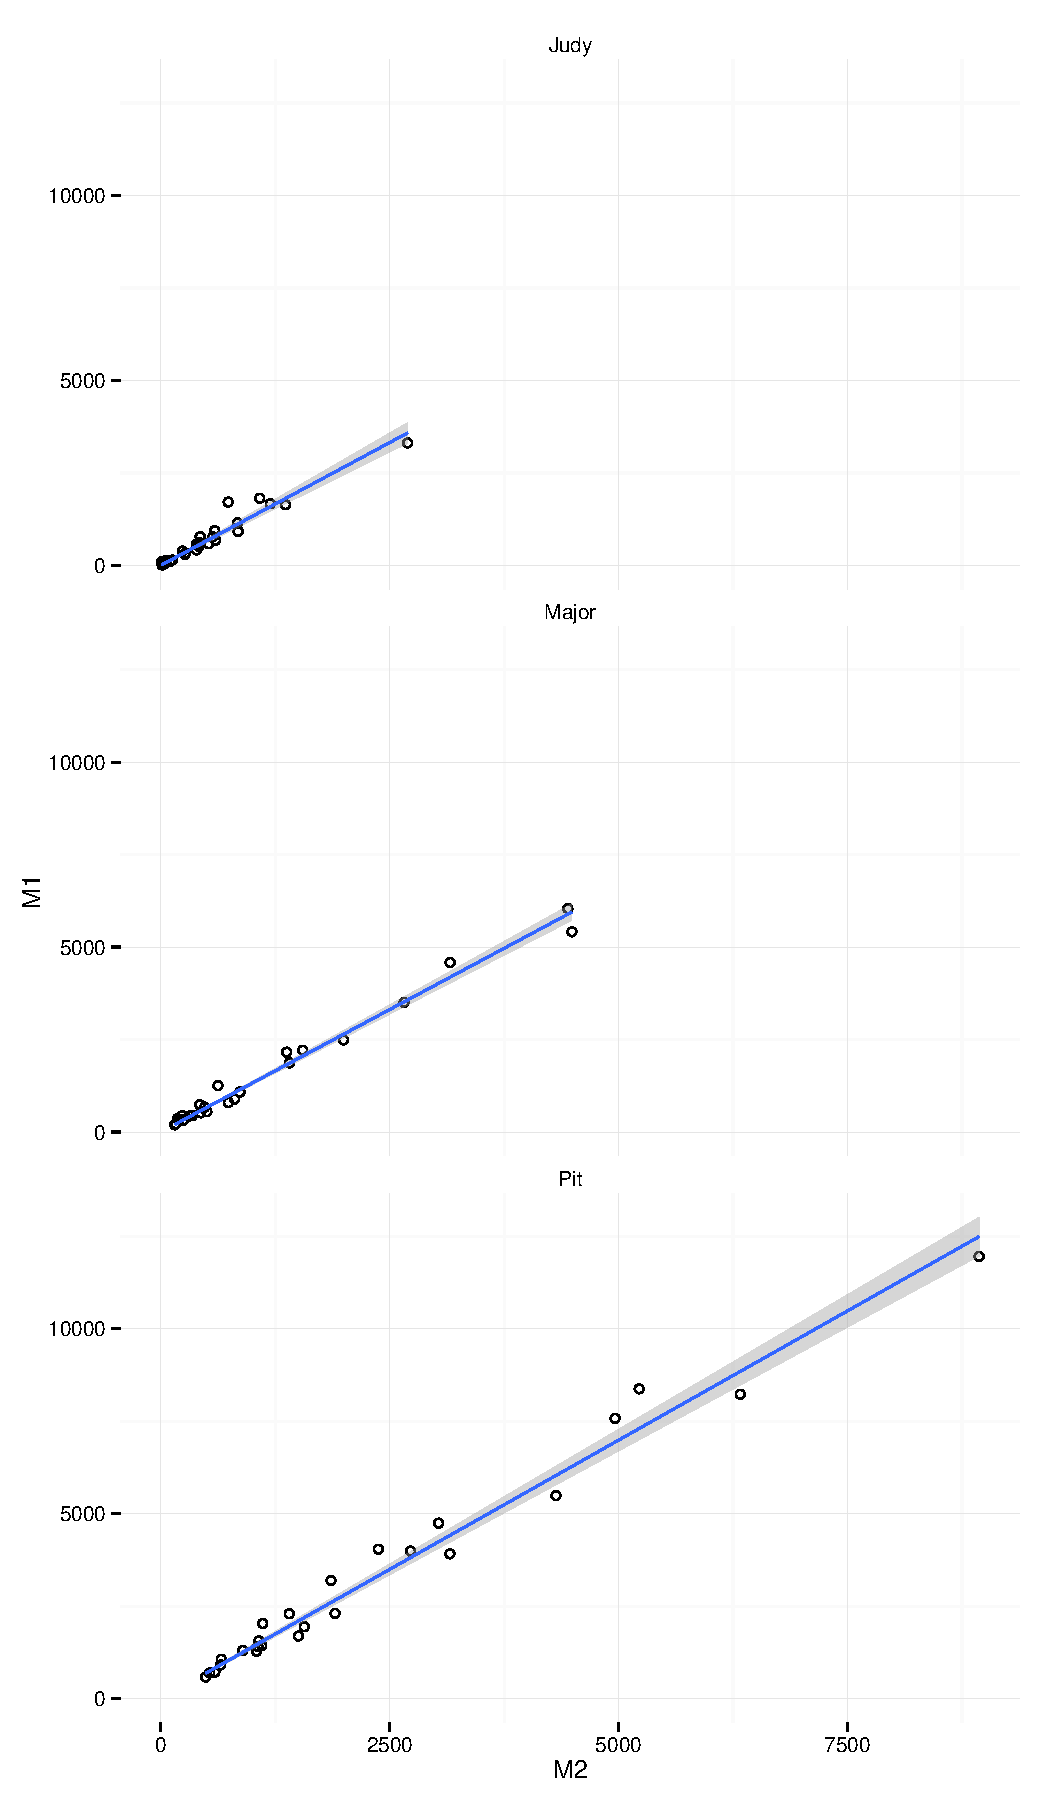
\includegraphics[width=.99\linewidth]{twocolumn-unnamed-chunk-7} 

}

\end{Schunk}

\caption{Plot $M_2 \times M_1$ for complete test suites. It can be seen that there is a strong
correlation between $M_2$ and $M_1$, irrespective of the project}
\label{fig:kill1}
\end{figure}




\begin{table}
\centering
\caption{Regression results for $M_2 \times M_1$ for complete test suites}
\centering
{\small
\begin{tabular}{rrrrr}
  \hline
 & Estimate & Std. Error & t value & Pr($>$$|$t$|$) \\ 
  \hline
m1 & 0.7085 & 0.0144 & 49.28 & 0.0000 \\ 
   \hline
\end{tabular}
}


\caption*{Pit $R^2=$0.99}
\centering
{\small
\begin{tabular}{rrrrr}
  \hline
 & Estimate & Std. Error & t value & Pr($>$$|$t$|$) \\ 
  \hline
m1 & 0.7491 & 0.0136 & 54.96 & 0.0000 \\ 
   \hline
\end{tabular}
}


\caption*{Major $R^2=$0.992}
\centering
{\small
\begin{tabular}{rrrrr}
  \hline
 & Estimate & Std. Error & t value & Pr($>$$|$t$|$) \\ 
  \hline
m1 & 0.7280 & 0.0274 & 26.55 & 0.0000 \\ 
   \hline
\end{tabular}
}


\caption*{Judy $R^2=$0.966}
\label{tbl:kill1}
\end{table}

\begin{table*}
\caption{Regression results for $M_{n+1}\times M_n$ for $\frac{1}{2^n}$ test suites}
\caption*{$R^2$}
  \begin{minipage}{.33\linewidth}
  \centering
{\small
\begin{tabular}{rrrrrrrr}
  \hline
 & 1 & $\frac{1}{2}$ & $\frac{1}{4}$ & $\frac{1}{8}$ & $\frac{1}{16}$ & $\frac{1}{32}$ & $\frac{1}{64}$ \\ 
  \hline
2x1 & 0.99 & 0.98 & 0.97 & 0.96 & 0.91 & 0.81 & 0.56 \\ 
  3x2 & 0.99 & 0.99 & 0.99 & 0.97 & 0.92 & 0.80 & 0.58 \\ 
  4x3 & 1.00 & 0.99 & 0.99 & 0.97 & 0.92 & 0.79 & 0.84 \\ 
  5x4 & 1.00 & 0.99 & 0.99 & 0.98 & 0.90 & 0.82 & 0.90 \\ 
  6x5 & 1.00 & 0.99 & 0.99 & 0.97 & 0.91 & 0.95 & 0.93 \\ 
  7x6 & 1.00 & 1.00 & 0.99 & 0.97 & 0.92 & 0.94 & 0.92 \\ 
  8x7 & 1.00 & 1.00 & 0.99 & 0.96 & 0.94 & 0.95 & 0.90 \\ 
  9x8 & 0.99 & 1.00 & 0.99 & 0.96 & 0.96 & 0.95 & 0.86 \\ 
  10x9 & 1.00 & 1.00 & 0.99 & 0.97 & 0.96 & 0.96 & 0.81 \\ 
   \hline
\end{tabular}
}


  \end{minipage}
  \begin{minipage}{.33\linewidth}
  \centering
{\small
\begin{tabular}{rrrrrrrr}
  \hline
 & 1 & $\frac{1}{2}$ & $\frac{1}{4}$ & $\frac{1}{8}$ & $\frac{1}{16}$ & $\frac{1}{32}$ & $\frac{1}{64}$ \\ 
  \hline
2x1 & 0.99 & 0.99 & 0.97 & 0.96 & 0.91 & 0.83 & 0.74 \\ 
  3x2 & 1.00 & 0.99 & 0.98 & 0.96 & 0.92 & 0.86 & 0.72 \\ 
  4x3 & 1.00 & 0.99 & 0.98 & 0.97 & 0.95 & 0.88 & 0.71 \\ 
  5x4 & 1.00 & 0.99 & 0.99 & 0.97 & 0.95 & 0.85 & 0.86 \\ 
  6x5 & 0.99 & 1.00 & 0.99 & 0.98 & 0.96 & 0.88 & 0.88 \\ 
  7x6 & 1.00 & 1.00 & 0.99 & 0.98 & 0.96 & 0.86 & 0.95 \\ 
  8x7 & 1.00 & 1.00 & 0.99 & 0.99 & 0.94 & 0.95 & 0.94 \\ 
  9x8 & 1.00 & 1.00 & 0.99 & 0.99 & 0.93 & 0.96 & 0.93 \\ 
  10x9 & 1.00 & 1.00 & 0.99 & 0.99 & 0.94 & 0.98 & 0.88 \\ 
   \hline
\end{tabular}
}


  \end{minipage}
  \begin{minipage}{.33\linewidth}
  \centering
{\small
\begin{tabular}{rrrrrrrr}
  \hline
 & 1 & $\frac{1}{2}$ & $\frac{1}{4}$ & $\frac{1}{8}$ & $\frac{1}{16}$ & $\frac{1}{32}$ & $\frac{1}{64}$ \\ 
  \hline
2x1 & 0.97 & 0.96 & 0.92 & 0.86 & 0.81 & 0.77 & 0.73 \\ 
  3x2 & 0.99 & 0.95 & 0.92 & 0.93 & 0.91 & 0.91 & 0.89 \\ 
  4x3 & 0.99 & 0.94 & 0.97 & 0.97 & 0.95 & 0.94 & 0.95 \\ 
  5x4 & 0.87 & 0.98 & 0.98 & 0.97 & 0.97 & 0.97 & 0.97 \\ 
  6x5 & 1.00 & 0.99 & 0.98 & 0.98 & 0.98 & 0.99 & 0.97 \\ 
  7x6 & 1.00 & 1.00 & 0.98 & 0.99 & 0.98 & 0.99 & 0.95 \\ 
  8x7 & 1.00 & 1.00 & 0.99 & 0.99 & 0.98 & 0.99 & 0.95 \\ 
  9x8 & 1.00 & 1.00 & 0.99 & 0.99 & 0.99 & 0.99 & 0.93 \\ 
  10x9 & 0.99 & 1.00 & 0.99 & 0.99 & 0.99 & 0.99 & 0.82 \\ 
   \hline
\end{tabular}
}


  \end{minipage}
\caption*{Estimate}
  \begin{minipage}{.33\linewidth}
  \centering
{\small
\begin{tabular}{rrrrrrrr}
  \hline
 & 1 & $\frac{1}{2}$ & $\frac{1}{4}$ & $\frac{1}{8}$ & $\frac{1}{16}$ & $\frac{1}{32}$ & $\frac{1}{64}$ \\ 
  \hline
2x1 & 0.71 & 0.65 & 0.58 & 0.50 & 0.42 & 0.33 & 0.22 \\ 
  3x2 & 0.80 & 0.75 & 0.69 & 0.63 & 0.56 & 0.49 & 0.39 \\ 
  4x3 & 0.85 & 0.80 & 0.75 & 0.72 & 0.66 & 0.59 & 0.62 \\ 
  5x4 & 0.87 & 0.82 & 0.80 & 0.77 & 0.72 & 0.69 & 0.66 \\ 
  6x5 & 0.87 & 0.84 & 0.83 & 0.80 & 0.77 & 0.81 & 0.67 \\ 
  7x6 & 0.91 & 0.87 & 0.85 & 0.82 & 0.82 & 0.81 & 0.66 \\ 
  8x7 & 0.90 & 0.89 & 0.87 & 0.84 & 0.86 & 0.80 & 0.64 \\ 
  9x8 & 0.86 & 0.90 & 0.88 & 0.86 & 0.89 & 0.78 & 0.59 \\ 
  10x9 & 0.91 & 0.91 & 0.89 & 0.88 & 0.88 & 0.80 & 0.56 \\ 
   \hline
\end{tabular}
}


\caption*{Pit}
  \end{minipage}
  \begin{minipage}{.33\linewidth}
  \centering
{\small
\begin{tabular}{rrrrrrrr}
  \hline
 & 1 & $\frac{1}{2}$ & $\frac{1}{4}$ & $\frac{1}{8}$ & $\frac{1}{16}$ & $\frac{1}{32}$ & $\frac{1}{64}$ \\ 
  \hline
2x1 & 0.75 & 0.68 & 0.59 & 0.51 & 0.44 & 0.37 & 0.29 \\ 
  3x2 & 0.81 & 0.74 & 0.69 & 0.66 & 0.61 & 0.52 & 0.38 \\ 
  4x3 & 0.84 & 0.79 & 0.76 & 0.76 & 0.70 & 0.57 & 0.46 \\ 
  5x4 & 0.86 & 0.82 & 0.83 & 0.80 & 0.73 & 0.60 & 0.65 \\ 
  6x5 & 0.87 & 0.86 & 0.86 & 0.83 & 0.75 & 0.65 & 0.70 \\ 
  7x6 & 0.88 & 0.88 & 0.88 & 0.84 & 0.76 & 0.70 & 0.80 \\ 
  8x7 & 0.91 & 0.90 & 0.89 & 0.85 & 0.75 & 0.82 & 0.78 \\ 
  9x8 & 0.89 & 0.92 & 0.90 & 0.86 & 0.76 & 0.85 & 0.76 \\ 
  10x9 & 0.93 & 0.93 & 0.91 & 0.86 & 0.79 & 0.89 & 0.70 \\ 
   \hline
\end{tabular}
}


\caption*{Major}
  \end{minipage}
  \begin{minipage}{.33\linewidth}
  \centering
{\small
\begin{tabular}{rrrrrrrr}
  \hline
 & 1 & $\frac{1}{2}$ & $\frac{1}{4}$ & $\frac{1}{8}$ & $\frac{1}{16}$ & $\frac{1}{32}$ & $\frac{1}{64}$ \\ 
  \hline
2x1 & 0.73 & 0.66 & 0.59 & 0.51 & 0.45 & 0.41 & 0.39 \\ 
  3x2 & 0.82 & 0.75 & 0.70 & 0.69 & 0.66 & 0.67 & 0.66 \\ 
  4x3 & 0.85 & 0.79 & 0.80 & 0.78 & 0.78 & 0.78 & 0.78 \\ 
  5x4 & 0.77 & 0.85 & 0.84 & 0.82 & 0.84 & 0.85 & 0.81 \\ 
  6x5 & 0.92 & 0.89 & 0.87 & 0.87 & 0.87 & 0.89 & 0.83 \\ 
  7x6 & 0.92 & 0.90 & 0.89 & 0.89 & 0.90 & 0.90 & 0.81 \\ 
  8x7 & 0.94 & 0.91 & 0.90 & 0.91 & 0.91 & 0.90 & 0.80 \\ 
  9x8 & 0.92 & 0.92 & 0.91 & 0.92 & 0.93 & 0.91 & 0.77 \\ 
  10x9 & 0.93 & 0.93 & 0.92 & 0.93 & 0.94 & 0.89 & 0.68 \\ 
   \hline
\end{tabular}
}


\caption*{Judy}
  \end{minipage}
\caption*{The row names indicate the ratios being examined, while columns indicate the fraction of test suite being considered}
\label{tbl:kille}
\end{table*}

Thus, we were left with three tools: PIT, Judy, and Major. We worked with the
authors of each to ensure that we had the latest version
(Judy 2.1.x, Major 1.1.5). For each tool, we used the settings to for the
maximum number of operators to mutate. In the case of PIT we extended PIT
to provide a more complete set of mutants, which were later accepted to the
main line (PIT 1.0).

Unlike other structural coverage measures such as statement, branch or path
coverage, there is very little agreement on what constitutes an acceptable
set of mutants in mutation analysis. This means that we can expect a wide
variation in the number of mutants produced. The number of mutants produced by each
tool on each program is given in Table~\ref{tbl:subjectsn}. Unfortunately,
this also means that the mutation scores do not necessarily agree as we
see in Table~\ref{tbl:subjects}. We removed mutants
that were not killed by any test cases we had, since our measure does not
include non-detected mutants. We then generated the full mutant kill matrix
for evaluation. Next, we randomized the mutation matrix 100
times, and generated the test cases-vice cumulative sum matrix from each\footnote{
For computing test case-vice cumulative sum matrix, we start with the matrix of
mutant kills (columns) vs test cases (rows). Then, starting from the second row,
we add the values in previous row to the values in current row to get the
current row. That is, at the last row, for each mutant, we have the total number
of times it was killed.
}.
Finally, we extracted the records at
$\{\frac{1}{2},\frac{1}{4},\frac{1}{8},\frac{1}{16},\frac{1}{32},\frac{1}{64}\}$
fractions of the full test suite size.

We perform our empirical analysis in two parts. In the first part, we consider all
the projects together, and derive a relation that is common across the projects.
In the second part, we consider Apache commons-math which has a mutation
adequate test suite, with $6,743$ tests of which $5,880$ killed at least one
mutant. Of the $122,484$ mutants generated, $89,631$ were killed by the test
suite, providing a mutation score of $73.18$\%. We consider this project in
detail, and show that our conclusions remain valid.






\begin{figure*}[!htb]
\begin{Schunk}


{\centering 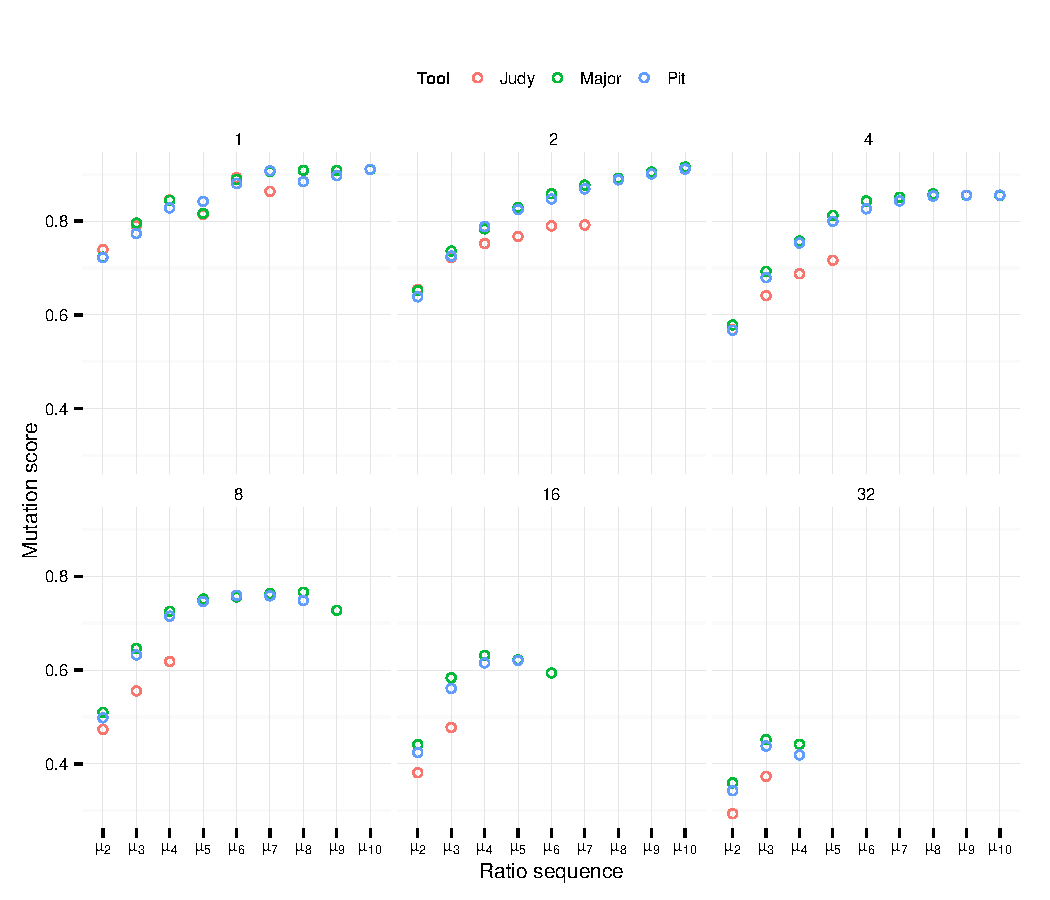
\includegraphics[width=.99\linewidth]{twocolumn-unnamed-chunk-23} 

}

\end{Schunk}

\caption{Progression of ratio $\frac{K_{i+1}}{K_i}$ in sequence $i$ for decreasing fractions
of the test suite. It can be seen here that for the smallest fraction of test suite ($\frac{1}{32}$), the ratio $\mu_2$ is very small, and the slope between $\mu_2$ and $\mu_3$ is large, with a very large curvature for the entire curve. As the test suite size increases from $\frac{1}{32}$ through $\frac{1}{16}$ to $\frac{1}{8}$ of the full test suite, we see that the slope decreases, and the curvature also decreases along with it. We see in $\frac{1}{4}$, $\frac{1}{2}$ and $1$ that the process of curvature straightening out and the difference between consecutive ratios decreasing to be almost none compared to what we started with. We expect the process to continue, and the curvature to reduce to zero for a perfectly mutation adequate test suite.}
\label{fig:tcfrac}
\end{figure*}


\section{Analysis}
The results of our two-part analysis are given below.
\subsection{All projects and tools}
We evaluate mutations from 25 projects using three tools:
Pit, Major, and Judy.
We first investigate the correlation between $M_2$ and $M_1$.
The plot of $M_2\times M_1$ across projects using their full test suite is given
in Figure~\ref{fig:kill1}. As can be seen, there is a very strong correlation
between $M_2$ and $M_1$ irrespective of the tool used across projects.

To investigate the actual relation between $M_2$ and $M_1$, we use linear
regression using the equation below.
\[
\mu\{M_2 | M_1\} = 0 + \beta_1 \times M_1
\]
We use zero intercept as we satisfy the two conditions of its use.
First, when there are no mutants that are killed by at least one test case,
there should not be any mutants that are killed by two. Secondly, we have
sufficient data near the origin.
The linear regression results are given in Table~\ref{tbl:kill1}. The results
confirm the very high correlation between the two measures irrespective of tool
used or project.
The relation between $M_2$ and $M_1$ is reflected in the relation
between other ratios.

The next question of interest is the impact of reduction of test suite size.
To evaluate this, we consider the various fractions of the full test suite,
randomly sampled. The sample fractions we investigated were
$\{\frac{1}{2},\frac{1}{4},\frac{1}{8},\frac{1}{16},\frac{1}{32},\frac{1}{64}\}$ of original test suite.
This is given in Table~\ref{tbl:kille} along with ratios from $\mu_2 = \frac{M_{2}}{M_{1}}$ through $\mu_{10} = \frac{M_{10}}{M_9}$.

Our observations on $M_{n+1}\times M_n$ across projects, and across differing
fractions of test suites shows that these measures are highly
correlated. High correlation between two variables essentially means that their
ratio is stable, and essentially same for any pair considered.
Hence, we can consider the mean of the ratio $\mu_2 = \frac{M_2}{M_1}$
(and $\mu_3 .. \mu_9$).

We plot the mean ratio $\mu_2$, $\mu_3$ through $\mu_{10}$ across all projects.
We compute the ratio for decreasing sizes of test suites, from using the entire
suite, to using only half the test suite, to using only $\frac{1}{32}$ of the
test suite. Figure~\ref{fig:tcfrac} captures the change in ratios as the test suite
sizes change. Note that not all projects are large enough to
provide $\frac{1}{64}$ test suite samples such that all $\mu_{n}$ scores could
be computed.
For Table~\ref{tbl:kille}, we ignored those tuples that did not exist.
However, for Figure~\ref{fig:tcfrac}, we plotted the mean values.
Since mean values tend to get skewed in favor of larger values when smaller
elements disappear, we preferred to plot only those test suite fractions
for which $\mu_{n}$ ratios were available for every project.

It can be seen that there is a large slope when the test suite is
largely inadequate at $\frac{1}{32}$ size of the original test suite size.
However, the slope reduces as the fraction size increases, with the least slope for
full size test suites. Note that the  behavior remains similar across all the
tested tools --- Pit, Judy, and Major.
\subsection{Analysis of Apache commons-math with Pit}
For an in-depth analysis of Apache commons-math, as before, we look at the
correlation for $M_2 \times M_1$. Figure~\ref{fig:amkill1} shows the
correlation between both.
The regression for $M_2\times M_1$ is given in Table~\ref{tbl:amkill1}.
\begin{table}
\centering
\caption{Regression results $M_2\times M_1$}
{\small
\begin{tabular}{rrrrr}
  \hline
 & Estimate & Std. Error & t value & Pr($>$$|$t$|$) \\ 
  \hline
m1 & 0.6649 & 0.0037 & 180.95 & 0.0000 \\ 
   \hline
\end{tabular}
}


\caption*{For Apache commons-math, complete test suite $R^2=$0.979}
\label{tbl:amkill1}
\end{table}
Similar to the across-projects evaluation, we also evaluate all the ratios
for Apache commons-math. Note that
unlike across-projects, we have only a single full test suite. Hence, the
comparison is given for randomly sampled $\frac{1}{2^n}$ test suite fractions ---
$\{\frac{1}{2},\frac{1}{4},\frac{1}{8},\frac{1}{16},\frac{1}{32},\frac{1}{64}\}$
of original test suite, which is given in Table~\ref{tbl:amkilln}.
\begin{table}
\centering
\caption{Regression results $M_2\times M_1$ for $\frac{1}{2^n}$ test suites -- Apache commons-math}
\caption*{$R^2$}
{\small
\begin{tabular}{rrrrrrr}
  \hline
 & $\frac{1}{2}$ & $\frac{1}{4}$ & $\frac{1}{8}$ & $\frac{1}{16}$ & $\frac{1}{32}$ & $\frac{1}{64}$ \\ 
  \hline
2x1 & 1.00 & 1.00 & 1.00 & 1.00 & 0.99 & 0.97 \\ 
  3x2 & 1.00 & 1.00 & 1.00 & 1.00 & 0.99 & 0.97 \\ 
  4x3 & 1.00 & 1.00 & 1.00 & 1.00 & 0.99 & 0.97 \\ 
  5x4 & 1.00 & 1.00 & 1.00 & 1.00 & 0.99 & 0.97 \\ 
  6x5 & 1.00 & 1.00 & 1.00 & 1.00 & 0.99 & 0.98 \\ 
  7x6 & 1.00 & 1.00 & 1.00 & 1.00 & 0.99 & 0.99 \\ 
  8x7 & 1.00 & 1.00 & 1.00 & 1.00 & 0.99 & 0.99 \\ 
  9x8 & 1.00 & 1.00 & 1.00 & 1.00 & 0.99 & 0.99 \\ 
  10x9 & 1.00 & 1.00 & 1.00 & 0.99 & 0.99 & 0.99 \\ 
   \hline
\end{tabular}
}


\caption*{Estimate}
{\small
\begin{tabular}{rrrrrrr}
  \hline
 & $\frac{1}{2}$ & $\frac{1}{4}$ & $\frac{1}{8}$ & $\frac{1}{16}$ & $\frac{1}{32}$ & $\frac{1}{64}$ \\ 
  \hline
2x1 & 0.68 & 0.61 & 0.55 & 0.47 & 0.39 & 0.30 \\ 
  3x2 & 0.77 & 0.73 & 0.68 & 0.62 & 0.54 & 0.45 \\ 
  4x3 & 0.82 & 0.79 & 0.75 & 0.69 & 0.62 & 0.56 \\ 
  5x4 & 0.86 & 0.83 & 0.78 & 0.73 & 0.67 & 0.61 \\ 
  6x5 & 0.88 & 0.84 & 0.81 & 0.77 & 0.72 & 0.68 \\ 
  7x6 & 0.89 & 0.86 & 0.83 & 0.78 & 0.73 & 0.72 \\ 
  8x7 & 0.90 & 0.87 & 0.85 & 0.80 & 0.77 & 0.77 \\ 
  9x8 & 0.91 & 0.88 & 0.87 & 0.82 & 0.80 & 0.79 \\ 
  10x9 & 0.92 & 0.89 & 0.87 & 0.83 & 0.82 & 0.81 \\ 
   \hline
\end{tabular}
}


\caption*{The rownames indicate the ratios being examined, while columns indicate the fraction of test suite being considered}
\label{tbl:amkilln}
\end{table}
Having shown that there is a high correlation between the sequence of
more and more strongly killed\footnote{Strongly killed just means killed by
more number of tests in this context.} mutants, and also having shown that
decreasing sample size does not affect the correlation, we can now examine the
ratio sequences across smaller and smaller test suites. This is given in
Figure~\ref{fig:amtcfrac}.
\begin{figure}
\begin{Schunk}


{\centering 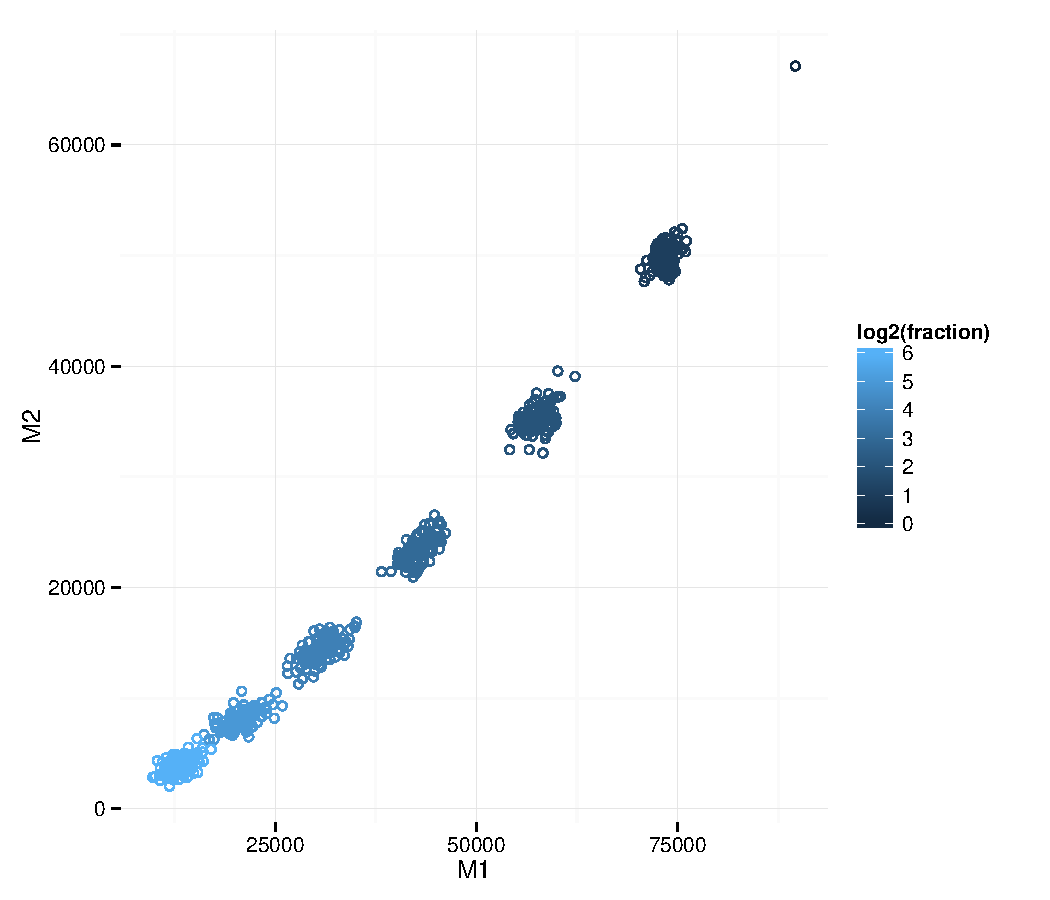
\includegraphics[width=.99\linewidth]{twocolumn-unnamed-chunk-21} 

}

\end{Schunk}

\caption{Plot of Apache commons-math $M_2\times M_1$ for $\frac{1}{2^n}$ test suites. The color is graded according to \emph{log(fraction)} of the test suite compared to full test suite. It can be seen that the ratio between $M_1$ and $M_2$ is consistent across different test suite strengths}
\label{fig:amkill1}
\end{figure}


\begin{figure*}
\begin{Schunk}


{\centering 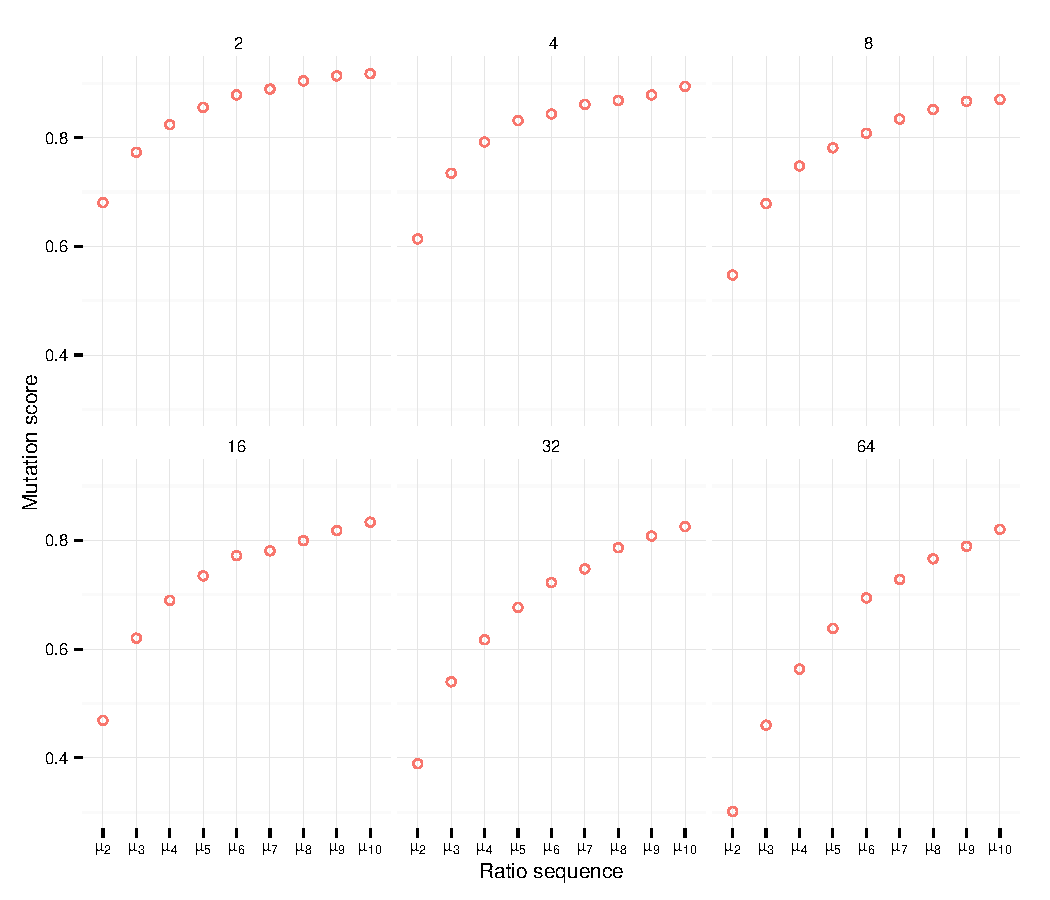
\includegraphics[width=.99\linewidth]{twocolumn-unnamed-chunk-24} 

}

\end{Schunk}

\caption{Progression of ratio $\frac{K_{i+1}}{K_i}$ in sequence $i$ for decreasing fractions
of the test suite for Apache commons-math.
It can be seen here that for the smallest fraction of test suite ($\frac{1}{64}$), the ratio $\mu_2$ is very small, and the slope between $\mu_2$ and $\mu_3$ is large, with a very large curvature for the entire curve. As the test suite size increases from $\frac{1}{64}$ through $\frac{1}{32}$ to $\frac{1}{16}$ of the full test suite, we see that the slope decreases, and the curvature also decreases along with it. We see in $\frac{1}{8}$, $\frac{1}{4}$ and $\frac{1}{2}$ that the process of curvature straightening out and the difference between consecutive ratios decreasing to be almost none compared to what we started with. We expect the process to continue, and the curvature to reduce to zero for a perfectly mutation adequate test suite.}
\label{fig:amtcfrac}
\end{figure*}





\section{Discussion}
\label{sec:discussion}

Our analysis reveals an interesting picture. As can be seen in Figure~\ref{fig:tcfrac},
the mean ratios between $\mu_1 .. \mu_{n}$ seem to follow a curve, with successive
$\mu_n$ ratios very close to the previous ones. The
successive ratios are closer to $1.0$, with the smallest ratios for $\mu_2$, and
the largest for $\mu_{10}$ where present. Secondly, the ratio $\mu_2$
is smallest for the smallest sized test suite ($\frac{1}{32}$ of the full test suite).
\greybox{
$N^{th}$ degree mutation scores ($\mu_n$) are very close to $(N+1)^{th}$ degree
mutation scores ($\mu_{n+1}$).
}
A very similar curve is found in an in-depth analysis of Apache commons-math
(Figure~\ref{fig:amtcfrac}). We find that the successive ratios become closer
to $1$ for $\frac{1}{2}$ test suite size (the trend is similar for the full
test suite, but we have a single data point for the full test suite, hence we
chose to not include it).

These two observations suggest that second degree mutation scores
($\mu_2$) become close to 1 (and close to first degree mutation
score --- $\mu_1$) when the test suite is adequate (and is
followed by successive ratios --- $\mu_3$, $\mu_4$
etc.). This suggests that second degree mutation score may be a reasonable
substitute for first degree mutation score ($\frac{M_1}{M_0}$) without its
disadvantages due to equivalent and redundant mutants.

\greybox{
The second degree mutation score $\mu_2 = \frac{M_2}{M_1}$ increases as test suite
adequacy increases.
}

It might indeed be possible to estimate the true first degree mutation score
from the second degree mutation score, by extrapolating the sequence curve
further to obtain $\frac{M_1}{M_0}$. Our data shows that the family of curves
is given by the function $odds(y) = \frac{y}{1-y}$ (Figure~\ref{fig:lines}).
However, the validation of this conjuncture requires a separate study for
identifying the equivalent mutants perhaps manually, and discounting their
influence.

A related observation is the relationship between test suite size and the
mutation score (Figure~\ref{fig:ts}).

\begin{table}
\centering
\caption{Regression between the fractional power of test suite size and $\mu_2$. l2f denotes the $log_2$ of the test suite fraction used.}
{\small
\begin{tabular}{rrrrr}
  \hline
 & Estimate & Std. Error & t value & Pr($>$$|$t$|$) \\ 
  \hline
(Intercept) & 0.7645 & 0.0082 & 92.94 & 0.0000 \\ 
  l2f & -0.0756 & 0.0021 & -35.78 & 0.0000 \\ 
   \hline
\end{tabular}
}


\caption*{$R^2$ = 0.996}
\label{tbl:ts}
\end{table}

\begin{figure}
\begin{Schunk}


{\centering 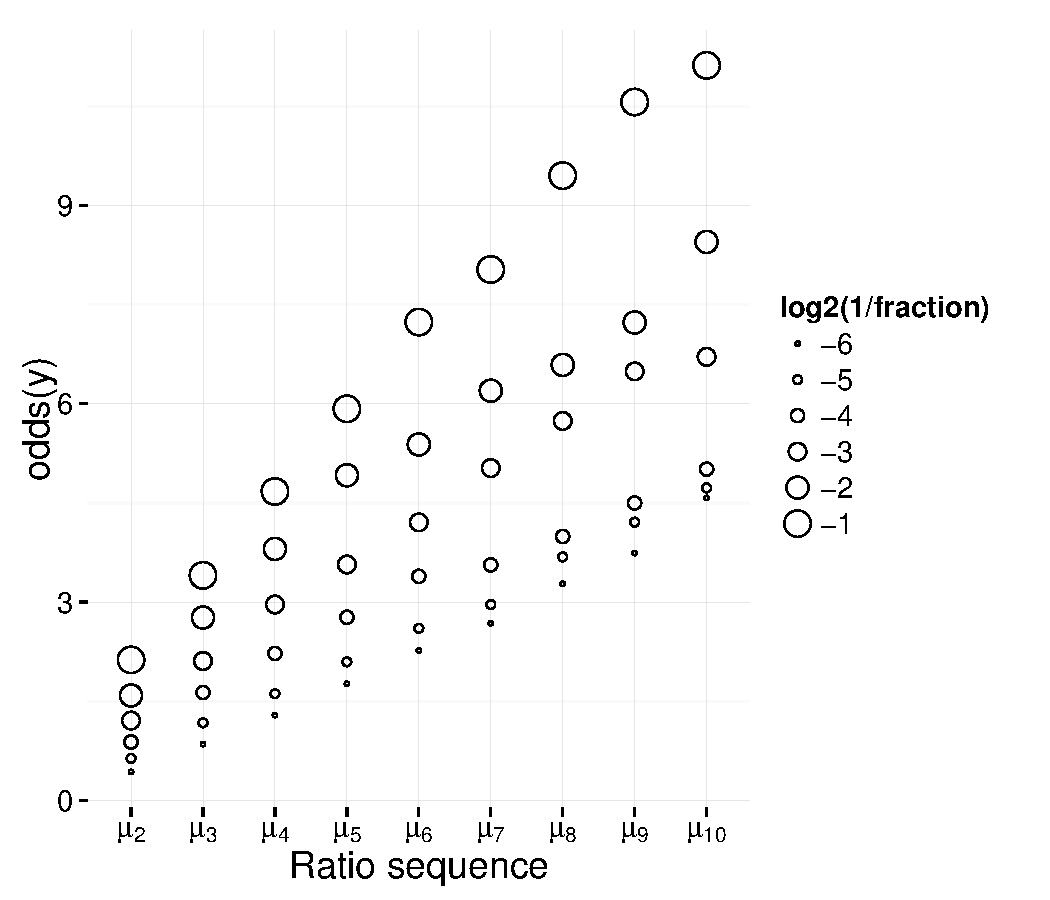
\includegraphics[width=.99\linewidth]{twocolumn-unnamed-chunk-26} 

}

\end{Schunk}

\caption{The family of curves can be represented by $odds(y) = \frac{y}{1-y}$ for Apache commons-math. It can be
seen that the increasing mutation ratios are almost perfectly captured by the odds ratio. We believe that
odds ratio can help us predict $\mu_1$ (the traditional mutation score) by
extrapolation of the lines. However, it requires further study.}
\label{fig:lines}
\begin{Schunk}


{\centering 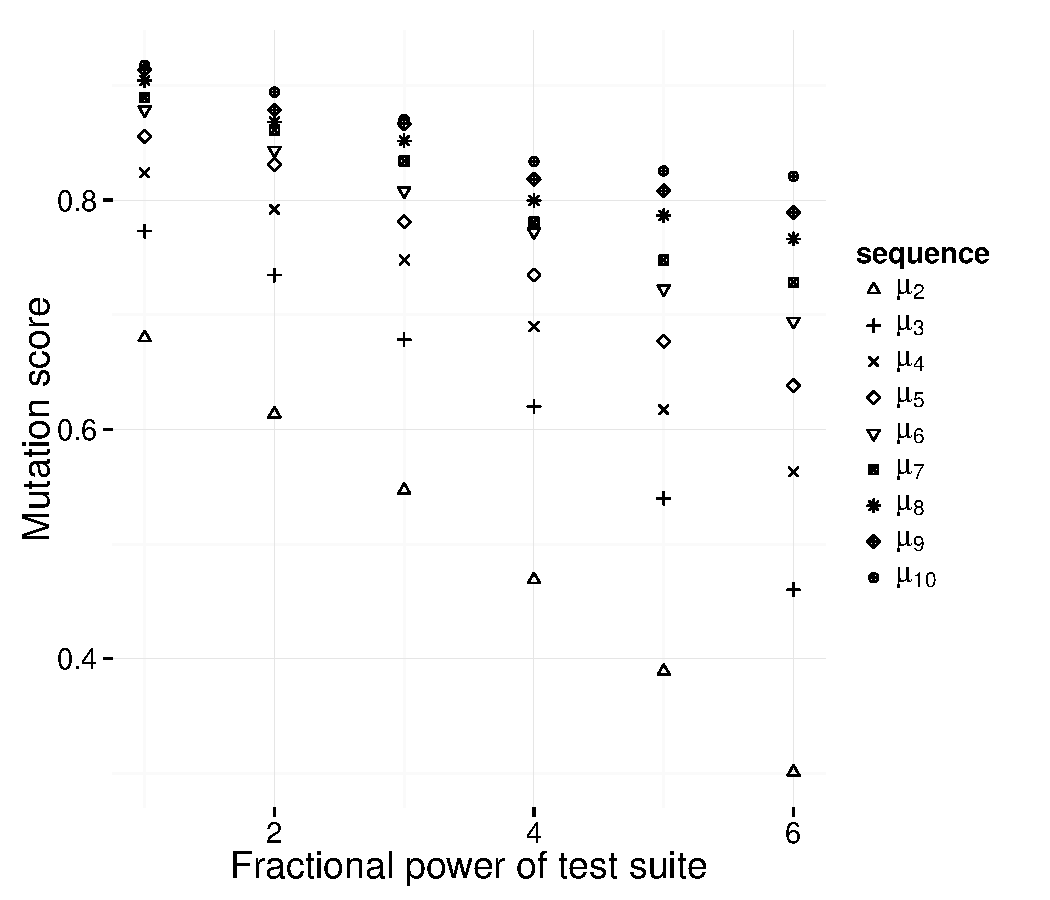
\includegraphics[width=.99\linewidth]{twocolumn-unnamed-chunk-27} 

}

\end{Schunk}

\caption{The relation between test suite size and mutation score for Apache commons-math.
For each doubling of test suite size, second degree mutation score increases by 0.076
points for Apache commons-math.}
\label{fig:ts}
\end{figure}
Our observations (Table~\ref{tbl:ts}) suggests that, for each doubling of test
suite size, second degree mutation score increases by 0.076
points for Apache commons-math.

What is the reason for the observed curve? The reason we see this particular curve
is that, at first, there is a fairly large difference between the number
of mutants that are killed by only one test case versus those killed by two,
and those killed by three etc. as we see in Figure~\ref{fig:amtcfrac}.
There are very few mutants that are killed by a large number of test cases, and
hence we can expect the ratio between higher
consecutive degrees to be closer to unity than the ratios between the lower
consecutive degrees of kills such as $M_1$ vs $M_2$. As newer test cases are
added, they contribute a few kills at higher degrees (moving a few mutants up),
while more kills are made at lower degrees. This means that the curve as a
whole rises up (see Figure~\ref{fig:amtcfrac} moving up from $\frac{1}{64}$ to
$\frac{1}{2}$). Since there is more impact on the lower degrees, as the curve
rises, it straightens, and levels out, with more and more test cases
contributing more to the lower degrees, and hence the ratio between lower
degrees decreasing faster, but the ratio between upper regions also decreasing.
Taken to the limit, we expect the curvature to approach zero for perfectly
mutation adequate test suites.

This is also the reason we can ignore the impact of redundant mutants. As we
see here, the decrease in curvature happens irrespective of the number of
redundant mutants involved, and the impact is such that their contribution is
accounted for in the shifting of the curvature.  Redundant mutants affect the
number of kills for each degree, but should not impact the ratios between the
degrees, unless redundant kills have an unexpected concentration of being
killed by a particular number of tests.



\section{Threats to Validity}
\label{sec:threats}

Our research makes use of multiple mutation tools, a variety of measures, and
numerous subjects. This means that our research is subject to the
following threats to validity.

The single most important threat to validity is the applicability of our
findings. Our subject programs were open source Java projects from Github.
While our choice of subjects was driven by concerns about the size of the
project (the larger the better), the size of the test suite (the larger
the better), and the ability to complete mutation analysis successfully
for the tools we selected, none of which  have any direct influence on the
measures, threats due to indirect unforeseen influences can't be ruled out.
Further, our research results are only directly applicable only to Java
programs. Though we expect our research to be applicable to mutation tools
in other programming languages too, there is no statistical guarantee for
such a belief other than the relative similarity between languages, between
possible bugs, and hence between mutants.

While we tried very hard to use different kinds of tools, the fact remains
that only three tools could be evaluated. This is not statistically adequate
for any sort of guarantee about the behavior of all tools. We base our
confidence on the observation that these tools are actively developed, used
by real world practitioners of testing and researchers, and also that the
mutation operators are reasonably complete. However, it is possible that
our tools may not be representative.

Finally, software bugs are a fact of life, and can't be ruled out either
in the tools used or in the analysis we performed.

While we have taken every care, the possibility of these threats remains.
Hence, it is important that our research be replicated for other languages
with different tools, and on tools using different phases for mutant
generation. To facilitate such efforts, we place the data from our
research and also the source code of our publication (which can be regenerated
from new data in the given format) online for easy access.




\section{Conclusion}
\label{sec:conclusion}

Our analysis suggests that second degree mutation score is a reliable
alternative for true mutation score, which avoids problems due to equivalent
and redundant mutants.   The second-degree mutation score for a test
suite is the ratio between mutants detected by at least two test cases
and mutants detected by at least one test case.  We have shown that the second degree
mutation score $\mu_2$ becomes equal to the traditional
mutation score $\mu_1$ when the test suite is adequate
(both evaluate to 1).

Our formulation avoids the problems of both equivalent and redundant mutants;
Equivalent mutants are avoided because the ratio $\mu_2 = \frac{M_2}{M_1}$
considers only those mutants that were killed at least once. We avoid the
problem due to redundant mutants by reformulating the concept of adequacy as
when the successive ratios $\mu_2, \mu_3 ..$ are
sufficiently close to 1 (which happens when $\mu_2$ is close to 1).

Our proposal for second degree mutation score trades some amount of runtime
efficiency for more accuracy in mutation analysis. It may be objected that mutation analysis
is already computationally intensive, and making it harder by requiring two kills rather than a
single kill makes mutation even less practical. However, we showed previously~\cite{gopinath2015howhard}
that sampling a constant number ($9,604$) of mutants can give a highly
accurate estimate of mutation score.  The same approach can be used
for second degree mutation, giving a constant (ignoring that test
suite size tends to grow with code size, a problem for all testing
methods, not just mutation) computational cost for even extremely
large projects.  Combining principle statistical sampling and second
degree mutation can provide a highly accurate measure of test suite
quality using mutants without an unreasonable computational demand.




\bibliographystyle{IEEEtran}
\bibliography{IEEEabrv,paper}

 



\end{document}
